% Beamer presentation - Hayashi & Koike (2020)
% M2 Gestion Quantitative II - Paris Dauphine - PSL
% Style rapproche du rendu Semestre 1.
% Compile with: pdflatex slide2.tex

\documentclass[10pt,aspectratio=169]{beamer}

\usetheme{Warsaw}
\usecolortheme{default}

\usepackage[utf8]{inputenc}
\usepackage[T1]{fontenc}
\usepackage[french]{babel}
\usepackage{amsmath,amssymb}
\usepackage{booktabs}
\usepackage{graphicx}
\usepackage{xcolor}

% ------------------------------------------------------------------
% Charte proche de la presentation du semestre 1
% ------------------------------------------------------------------
\definecolor{DauphineBlue}{RGB}{48,48,180}
\definecolor{DauphineBlueDark}{RGB}{25,38,120}
\definecolor{DauphineBlueLight}{RGB}{229,235,255}
\definecolor{TextGrey}{RGB}{55,55,65}

\setbeamercolor{structure}{fg=DauphineBlue}
\setbeamercolor{palette primary}{bg=DauphineBlue,fg=white}
\setbeamercolor{palette secondary}{bg=DauphineBlueDark,fg=white}
\setbeamercolor{palette tertiary}{bg=DauphineBlue,fg=white}
\setbeamercolor{palette quaternary}{bg=DauphineBlueDark,fg=white}
\setbeamercolor{title}{fg=white,bg=DauphineBlue}
\setbeamercolor{frametitle}{fg=white,bg=DauphineBlue}
\setbeamercolor{block title}{bg=DauphineBlue,fg=white}
\setbeamercolor{block body}{bg=DauphineBlueLight,fg=TextGrey}
\setbeamercolor{normal text}{fg=TextGrey,bg=white}

\setbeamertemplate{navigation symbols}{}
\setbeamertemplate{footline}{
  \leavevmode%
  \hbox{%
    \begin{beamercolorbox}[wd=.72\paperwidth,ht=2.5ex,dp=1ex,leftskip=1em]{palette primary}
      \usebeamerfont{author in head/foot}\insertshortauthor
    \end{beamercolorbox}%
    \begin{beamercolorbox}[wd=.28\paperwidth,ht=2.5ex,dp=1ex,rightskip=1em plus1fil]{palette secondary}
      \usebeamerfont{date in head/foot}\insertframenumber{} / \inserttotalframenumber
    \end{beamercolorbox}%
  }%
  \vskip0pt%
}
\setbeamertemplate{blocks}[rounded][shadow=true]
\setbeamertemplate{itemize item}{\color{DauphineBlue}$\blacktriangleright$}
\setbeamertemplate{itemize subitem}{\color{DauphineBlueDark}$\bullet$}

\title[Hayashi--Koike lead-lag HF]{Multi-scale analysis of lead-lag relationships\\in high-frequency financial markets}
\subtitle{Réplication méthodologique et application sur données 2025--2026}
\author[Renault \; Verdelhan \; El Arari]{Léo Renault \and Théo Verdelhan \and Ziad El Arari}
\institute[Paris-Dauphine PSL]{Master 2 -- Ingénierie Économique et Financière\\Parcours Finance Quantitative\\Université Paris-Dauphine -- PSL}
\date{2026}

\newcommand{\thetahat}{\hat{\theta}}
\newcommand{\Uhat}{\hat{U}}
\newcommand{\Gammahat}{\hat{\Gamma}}
\newcommand{\Psij}{\Psi_j}
\newcommand{\R}{\mathbb{R}}
\newcommand{\E}{\mathbb{E}}

\AtBeginSection[]{
  \begin{frame}{Plan}
    \tableofcontents[currentsection]
  \end{frame}
}

\begin{document}

\begin{frame}
  \titlepage
\end{frame}

\begin{frame}{Auteurs de l'article}
  \begin{block}{Article étudié}
    Hayashi, T. et Koike, Y. (2020), \emph{Multi-scale analysis of lead-lag relationships in high-frequency financial markets}.
  \end{block}

  \vspace{0.35cm}
  \begin{columns}[T]
    \begin{column}{0.48\linewidth}
      \textbf{Takaki Hayashi}
      \begin{itemize}
        \item Keio University
        \item Graduate School of Business Administration
      \end{itemize}
    \end{column}
    \begin{column}{0.48\linewidth}
      \textbf{Yuta Koike}
      \begin{itemize}
        \item University of Tokyo
        \item Graduate School of Mathematical Sciences
      \end{itemize}
    \end{column}
  \end{columns}

  \vspace{0.35cm}
  \small L'article propose un estimateur de lead-lag par échelle de temps, adapté aux données haute fréquence non synchrones.
\end{frame}

\begin{frame}{Plan}
  \begin{enumerate}
    \item Contexte, motivation et contribution de l'étude
    \item Modèle et estimateur Hayashi--Koike
    \item Implémentation indépendante
    \item Données et pré-traitements
    \item Validation de l'estimateur
    \item Résultat central : même actif, deux venues
    \item Comparaisons et extensions
    \item Limites et conclusion
  \end{enumerate}
\end{frame}

% ============================================================
\section{Contexte et motivation}
% ============================================================

\begin{frame}{Introduction : réplication + objectifs}
  \begin{itemize}
    \item Le papier étudie le \textbf{lead-lag} : un marché ou un actif peut incorporer l'information avant un autre.
    \item En haute fréquence, ce n'est pas un simple problème de corrélation :
      \begin{itemize}
        \item les observations ne sont pas synchrones ;
        \item les prix sont bruités par la microstructure ;
        \item le lag peut changer selon l'horizon observé.
      \end{itemize}
    \item Notre objectif : réimplémenter l'estimateur de manière autonome, puis l'appliquer à des données récentes exploitables.
  \end{itemize}
\end{frame}

\begin{frame}{Question économique}
  \begin{block}{Question du papier}
    Le leader est-il le même à très court horizon et à horizon un peu plus long ?
  \end{block}

  \vspace{0.25cm}
  \begin{itemize}
    \item À l'échelle sub-millisecondes : latence, ordre des quotes, conventions d'horodatage.
    \item À l'échelle millisecondes / secondes : arbitrage, découverte de prix, réaction du carnet.
    \item Un estimateur unique peut mélanger ces mécanismes.
  \end{itemize}

  \vspace{0.25cm}
  \textbf{Apport HK :} estimer un lag \(\theta_j\) différent pour chaque échelle \(j\).
\end{frame}

\begin{frame}{Limites de l'interpolation}
  \begin{block}{Interpolation sur grille}
    Interpoler les deux prix sur une grille régulière, puis calculer une corrélation retardée.
  \end{block}

  \vspace{0.25cm}
  \begin{itemize}
    \item On fabrique des prix qui n'ont pas été réellement observés.
    \item Le résultat dépend fortement du pas de grille choisi.
    \item À haute fréquence, l'effet Epps et le bid-ask bounce peuvent dominer le signal.
  \end{itemize}

  \vspace{0.25cm}
  HK évitent cette étape : ils travaillent directement avec les intervalles d'observation.
\end{frame}

\begin{frame}{Apport de Hayashi--Koike}
  \begin{itemize}
    \item \textbf{Hayashi--Yoshida} : mesurer une covariance sans imposer une grille commune.
    \item \textbf{Ondelettes} : séparer le signal par bandes de fréquence.
    \item \textbf{Argmax par échelle} : extraire un lead-lag \(\thetahat_j\) pour chaque horizon.
  \end{itemize}

  \vspace{0.3cm}
  \begin{exampleblock}{Idée clé}
    HK ne cherchent pas ``le'' lead-lag. Ils cherchent une courbe de lead-lag selon l'échelle.
  \end{exampleblock}
\end{frame}

\begin{frame}{Où se place le papier dans le cours}
  \small
  \begin{tabular}{p{0.28\linewidth}p{0.62\linewidth}}
    \toprule
    \textbf{Notion du cours} & \textbf{Utilisation dans HK} \\
    \midrule
    Ondelettes, Daubechies & Filtre passe-bande pour isoler les échelles. \\
    Covariance multirésolution & Point de départ : covariance par échelle. \\
    Lead-lag multi-échelle & HK formalise l'argmax du lag au lieu d'un décalage manuel. \\
    Microstructure HF & Non-synchronicité, latence, quote vs trade. \\
    \bottomrule
  \end{tabular}
\end{frame}

% ============================================================
\section{Méthode HK}
% ============================================================

\begin{frame}{Modèle : une corrélation différente par échelle}
  \small
  HK modélisent deux Brownien corrélés, avec une densité cross-spectrale par bandes :
  \[
    f_N(\lambda)
    =
    \sum_{j=1}^{N+1}
    R_j e^{-i\lambda\theta_j}
    \mathbf{1}_{\Lambda_{N-j+1}}(\lambda).
  \]

  \vspace{0.2cm}
  \begin{itemize}
    \item \(R_j\) : intensité de dépendance à l'échelle \(j\).
    \item \(\theta_j\) : décalage temporel à cette échelle.
    \item Les log-prix observés peuvent avoir une volatilité stochastique :
    \[
      X_t^\nu = X_0^\nu + \int_0^t \sigma_s^\nu dB_s^\nu .
    \]
  \end{itemize}
\end{frame}

\begin{frame}{Étape 1 : covariance Hayashi--Yoshida laggée}
  Pour un lag \(\tau\), on décale la deuxième série et on somme les produits d'incréments qui se chevauchent :
  \[
    \Uhat_N(\tau)
    =
    \sum_{I \in \mathcal{O}^1,\; J \in \mathcal{O}^2}
    \Delta X^1(I)\Delta X^2(J)
    \mathbf{1}_{I \cap (J+\tau) \neq \emptyset}.
  \]

  \vspace{0.25cm}
  \begin{itemize}
    \item C'est la brique qui gère la non-synchronicité.
    \item Aucun previous-tick obligatoire.
    \item Dans notre code : \(\thetahat_j>0\) signifie que la série 2 leade la série 1.
  \end{itemize}
\end{frame}

\begin{frame}{Étape 2 : filtrer par ondelette}
  À chaque échelle \(j\), HK filtrent la covariance laggée :
  \[
    \Gammahat_j(\tau)
    =
    \sum_{\ell}
    \Uhat_N(\tau-\ell\Delta_N)\Psij(\ell).
  \]

  \vspace{0.25cm}
  \begin{itemize}
    \item \(\Psij\) est l'autocorrélation d'un filtre de Daubechies.
    \item \(\Delta_N\) fixe la résolution des lags et les bandes temporelles.
  \end{itemize}
\end{frame}

\begin{frame}{Étape 3 : récupérer le lag}
  Le lag estimé à l'échelle \(j\) est le maximum du contraste :
  \[
    \thetahat_j
    =
    \arg\max_{\tau \in G_N}
    |\Gammahat_j(\tau)|.
  \]

  \vspace{0.25cm}
  \begin{columns}[T]
    \begin{column}{0.47\linewidth}
      \textbf{HRY single-scale}
      \begin{itemize}
        \item un seul lag ;
        \item plus simple à lire ;
        \item peut annuler deux effets opposés.
      \end{itemize}
    \end{column}
    \begin{column}{0.47\linewidth}
      \textbf{HK multi-échelle}
      \begin{itemize}
        \item un lag par \(j\) ;
        \item sépare plusieurs horizons ;
        \item plus proche du message du papier.
      \end{itemize}
    \end{column}
  \end{columns}
\end{frame}

\begin{frame}{Résultat empirique du papier HK}
  \small
  HK appliquent leur méthode à 108 actions du NASDAQ-100, août 2015, en comparant pour chaque action NASDAQ et BATS.

  \vspace{0.25cm}
  \begin{tabular}{p{0.32\linewidth}p{0.56\linewidth}}
    \toprule
    \textbf{Échelles fines} & Pic positif autour de \(+0.2\) à \(+0.3\) ms : NASDAQ leade BATS, proche du mécanisme DS. \\
    \midrule
    \textbf{Échelles plus larges} & Distribution plus hétérogène, souvent négative : BATS leade NASDAQ sur une partie du panel, proche du mécanisme HRY. \\
    \bottomrule
  \end{tabular}

  \vspace{0.35cm}
  \normalsize
  Le point important n'est pas ``NASDAQ gagne'' ou ``BATS gagne'', mais la séparation de deux mécanismes à deux horizons.
\end{frame}

% ============================================================
\section{Implémentation}
% ============================================================

\begin{frame}{Contrôle de signe}
  \begin{block}{Test synthétique}
    On construit deux séries où la série 1 leade la série 2 de \(+3\) secondes.
  \end{block}

  \vspace{0.25cm}
  L'estimateur retourne :
  \[
    \thetahat_{\text{HY}} \simeq -3,
    \qquad
    \thetahat_{\text{HK}} \simeq -3.
  \]

  \vspace{0.25cm}
  \begin{itemize}
    \item Convention interne : \(\thetahat_j < 0 \Leftrightarrow\) série 1 leade série 2.
    \item Donc \(\thetahat_j > 0 \Leftrightarrow\) série 2 leade série 1.
  \end{itemize}
\end{frame}

% ============================================================
\section{Données}
% ============================================================

\begin{frame}{Exigence de données}
  \begin{itemize}
    \item Consigne du projet : travailler sur données réelles, idéalement 2025--2026.
    \item Problème : le protocole exact HK est difficilement accessible publiquement :
      \begin{itemize}
        \item quotes NASDAQ/BATS ;
        \item micro-prices ;
        \item timestamps SIP et participant ;
        \item panel complet d'août 2015.
      \end{itemize}
    \item Choix pratique : garder la méthode HK et utiliser des données haute fréquence disponibles.
  \end{itemize}
\end{frame}

\begin{frame}{Papier HK vs notre périmètre de données}
  \small
  \begin{tabular}{p{0.22\linewidth}p{0.33\linewidth}p{0.33\linewidth}}
    \toprule
    & \textbf{Hayashi--Koike} & \textbf{Application locale} \\
    \midrule
    Actifs & 108 actions NASDAQ-100 & Crypto (BTC, ETH) \\
    Setup & Même action, NASDAQ vs BATS & Cross-venue / cross-product / cross-asset \\
    Prix & Micro-prices de quotes & Trades crypto (aggTrades) \\
    Période & Août 2015 & Principalement 2025--2026 \\
    Résolution & \(\sim 0.1\) ms & 50 ms (crypto) \\
    \bottomrule
  \end{tabular}
\end{frame}

\begin{frame}{Sources de données}
  \small
  \begin{tabular}{p{0.24\linewidth}p{0.28\linewidth}p{0.36\linewidth}}
    \toprule
    \textbf{Source} & \textbf{Format} & \textbf{Usage} \\
    \midrule
    Binance Vision & aggTrades, parquet cache & Spot, USDT-M perp, COIN-M perp. \\
    Bybit archive & CSV.gz trades & Cross-exchange spot. \\
    Kraken REST & trades paginés & Cross-exchange spot, même asset. \\
    Hyperliquid live & snapshots L2 & Piste future pour vrais micro-prices crypto. \\
    \bottomrule
  \end{tabular}

  \vspace{0.35cm}
  \normalsize
  Toutes les sources sont transformées en un même objet : deux séries de log-prix non synchrones.
\end{frame}

\begin{frame}{Prix : transaction vs micro-price}
  \begin{itemize}
    \item HK utilisent un micro-price de carnet :
    \[
      P^{micro}
      =
      \frac{P^{ask}V^{bid}+P^{bid}V^{ask}}
      {V^{bid}+V^{ask}}.
    \]
    \item Sur crypto historique public, le carnet complet est souvent absent ou payant.
    \item On utilise donc le \textbf{log-prix de transaction} (aggTrades) comme prix.
  \end{itemize}
\end{frame}

\begin{frame}{Pré-traitements}
  \begin{enumerate}
    \item Télécharger ou lire les fichiers bruts par jour.
    \item Convertir les timestamps en secondes Unix.
    \item Détecter automatiquement les timestamps Binance en ms ou \(\mu s\).
    \item Trier et dédupliquer les timestamps répétés.
    \item Passer les prix en log-prix.
    \item Construire une \texttt{NonSyncSeries} commune à tous les estimateurs.
  \end{enumerate}

  \vspace{0.35cm}
  \begin{exampleblock}{Point important}
    \(\Delta_N\) ne sert pas à interpoler les prix : il sert à définir la grille de lags et les échelles wavelet.
  \end{exampleblock}
\end{frame}

\begin{frame}{Même méthode, horizons différents}
  \small
  \begin{center}
  \begin{tabular}{ccc}
    \toprule
    \textbf{Échelle} & \textbf{HK 2020} & \textbf{Notre application} \\
    \midrule
    \(j=1\) & 0.2--0.4 ms & 0.10--0.20 s \\
    \(j=4\) & 1.6--3.2 ms & 0.80--1.60 s \\
    \(j=6\) & 6.4--12.8 ms & 3.20--6.40 s \\
    \(j=8\) & -- & 12.80--25.60 s \\
    \bottomrule
  \end{tabular}
  \end{center}

  \vspace{0.35cm}
  \begin{exampleblock}{Lecture}
    On conserve la logique multi-échelle de HK, mais pas le régime ultra-millisecondes du papier.
  \end{exampleblock}
\end{frame}

\begin{frame}{Non-synchronicité du cas central}
  \small
  \begin{columns}[T]
    \begin{column}{0.46\linewidth}
      \textbf{BTC, avril 2026}
      \vspace{0.15cm}

      \begin{tabular}{lrr}
        \toprule
        & \textbf{Trades} & \textbf{Inter-tick médian} \\
        \midrule
        Binance & 12.6 M & 32.5 ms \\
        Kraken & 0.86 M & 1.39 s \\
        \bottomrule
      \end{tabular}
    \end{column}
    \begin{column}{0.48\linewidth}
      \begin{block}{Conséquence}
        Le ratio de cadence médian est d'environ \(43\times\). Un alignement sur grille donnerait beaucoup de prix artificiels côté Kraken.
      \end{block}

    \end{column}
  \end{columns}
\end{frame}

% ============================================================
\section{Validation}
% ============================================================

\begin{frame}{Validation : trois contrôles}
  \scriptsize
  \begin{tabular}{p{0.25\linewidth}p{0.29\linewidth}p{0.24\linewidth}p{0.15\linewidth}}
    \toprule
    \textbf{Contrôle} & \textbf{Vérité injectée} & \textbf{Résultat} & \textbf{Rôle} \\
    \midrule
    Signe HY/HK & Série 1 mène série 2 de \(+3\) s & \(\hat\theta \simeq -3.00\) s & Convention \\
    Monte Carlo db10 & \((1,1,2,2,3,5,7,10)\Delta_N\) & \(j=1..4\) bien récupérés & Méthode HK \\
    Densité de ticks & Sous-échantillonnage asymétrique & 15/16 cellules gardent le bon signe & Artefact simple \\
    \bottomrule
  \end{tabular}

  \vspace{0.45cm}
  \begin{exampleblock}{Convention affichée}
    Dans nos tableaux, \(\hat\theta_j < 0\) signifie que la série 1 mène la série 2 ; \(\hat\theta_j > 0\) signifie que la série 2 mène la série 1.
  \end{exampleblock}
\end{frame}

\begin{frame}{Monte Carlo : portée de la validation}
  \begin{itemize}
    \item Le papier valide l'estimateur sur \(n=30000\) et 1000 trajectoires.
    \item Notre simulation est plus légère : \(n=8192\), 20 trajectoires.
    \item Ce qu'il valide correctement : les échelles fines et l'avantage du non-synchrone sur l'interpolation.
    \item Ce qu'on ne revendique pas : une reproduction numérique des Tables 2--3 du papier.
  \end{itemize}

  \vspace{0.35cm}
  \begin{block}{Positionnement}
    La validation sert à vérifier la mécanique de l'estimateur avant les données réelles.
  \end{block}
\end{frame}

% ============================================================
\section{Résultat central}
% ============================================================

\begin{frame}{BTC Binance/Kraken : le résultat central}
  \begin{columns}[T]
    \begin{column}{0.66\linewidth}
      \centering
      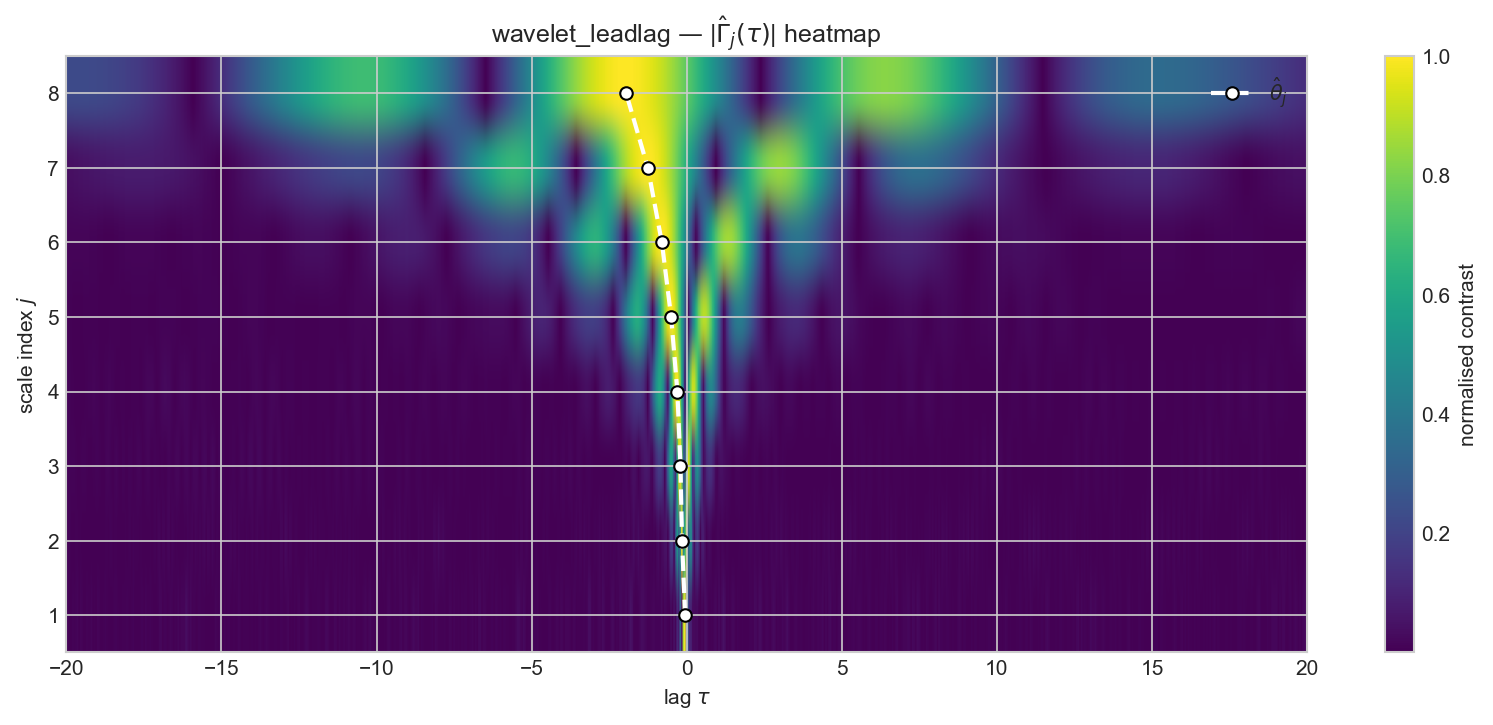
\includegraphics[width=\linewidth,height=0.68\textheight,keepaspectratio]{figures/heatmap_btc_binance_vs_kraken_full_month.png}
    \end{column}
    \begin{column}{0.30\linewidth}
      \small
      \begin{block}{Avril 2026}
        Même actif, deux venues : le cas le plus proche de NASDAQ/BATS.
      \end{block}

      \vspace{0.15cm}
      \begin{tabular}{lrr}
        \toprule
        \(j\) & \textbf{Horizon} & \(\hat\theta_j\) \\
        \midrule
        1 & 0.1--0.2 s & -0.05 s \\
        4 & 0.8--1.6 s & -0.30 s \\
        6 & 3.2--6.4 s & -0.80 s \\
        8 & 12.8--25.6 s & -1.95 s \\
        \bottomrule
      \end{tabular}

      \vspace{0.15cm}
      \textbf{Lecture :} Binance mène Kraken, et l'amplitude augmente avec l'échelle.
    \end{column}
  \end{columns}
\end{frame}

\begin{frame}{Robustesse temporelle}
  \begin{columns}[T]
    \begin{column}{0.62\linewidth}
      \centering
      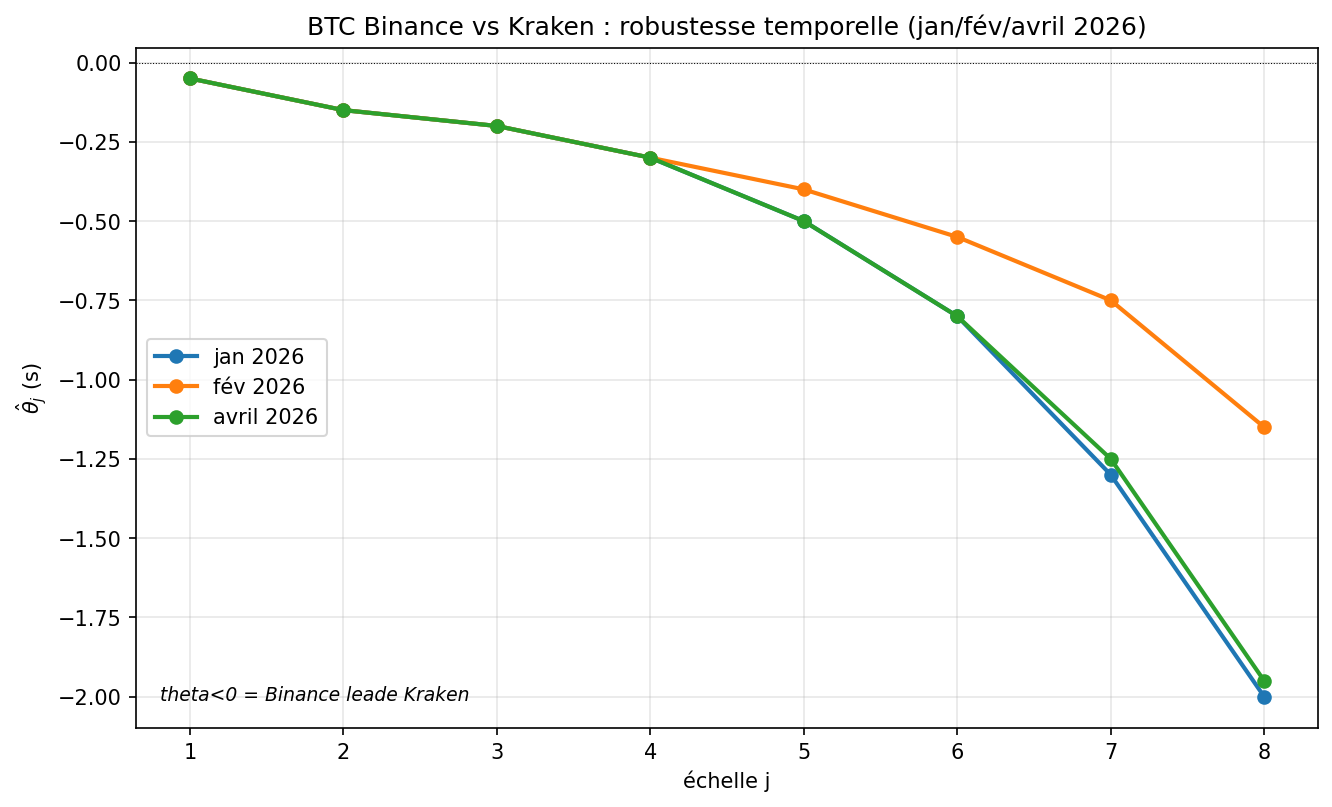
\includegraphics[width=\linewidth,height=0.66\textheight,keepaspectratio]{figures/temporal_panel_btc_binance_vs_kraken.png}
    \end{column}
    \begin{column}{0.34\linewidth}
      \small
      \begin{tabular}{lrr}
        \toprule
        \textbf{Mois} & \(\hat\theta_6\) & \(\hat\theta_8\) \\
        \midrule
        Jan. 2026 & -0.80 s & -2.00 s \\
        Fév. 2026 & -0.55 s & -1.15 s \\
        Avr. 2026 & -0.80 s & -1.95 s \\
        \bottomrule
      \end{tabular}

      \vspace{0.35cm}
      \begin{block}{Résultat}
        La direction est stable : \(\hat\theta_j < 0\) sur les trois mois.
      \end{block}

      \vspace{0.1cm}
      La magnitude est plus faible en février : effet de régime, pas inversion du signal.
    \end{column}
  \end{columns}
\end{frame}

\begin{frame}{Panel 30 jours : trois régularités}
  \begin{columns}[T]
    \begin{column}{0.63\linewidth}
      \centering
      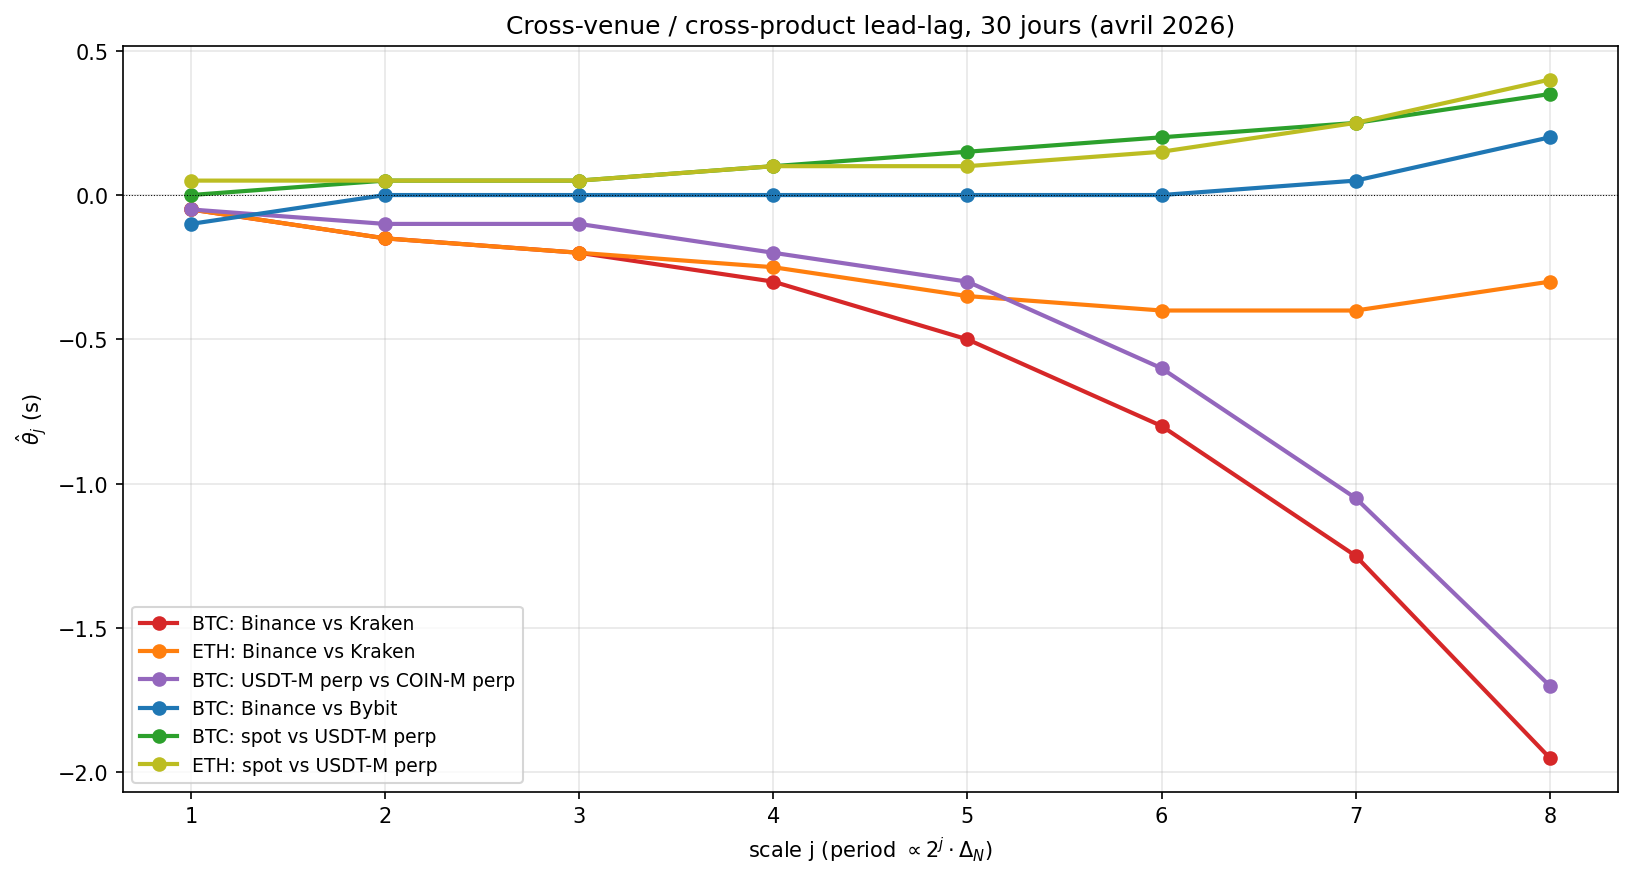
\includegraphics[width=\linewidth,height=0.68\textheight,keepaspectratio]{figures/comparison_panel_full_month.png}
    \end{column}
    \begin{column}{0.33\linewidth}
      \small
      \begin{enumerate}
        \item Binance mène Kraken sur BTC et ETH.
        \item USDT-M mène COIN-M sur le perp BTC.
        \item Le perpétuel mène le spot sur BTC et ETH.
      \end{enumerate}

      \vspace{0.25cm}
      \begin{block}{Synthèse}
        Le signal le plus propre reste le cross-venue même actif.
      \end{block}
    \end{column}
  \end{columns}
\end{frame}

% ============================================================
\section{Comparaisons et extensions}
% ============================================================

\begin{frame}{HK vs HRY : apport du multi-échelle}
  \begin{columns}[T]
    \begin{column}{0.68\linewidth}
      \centering
      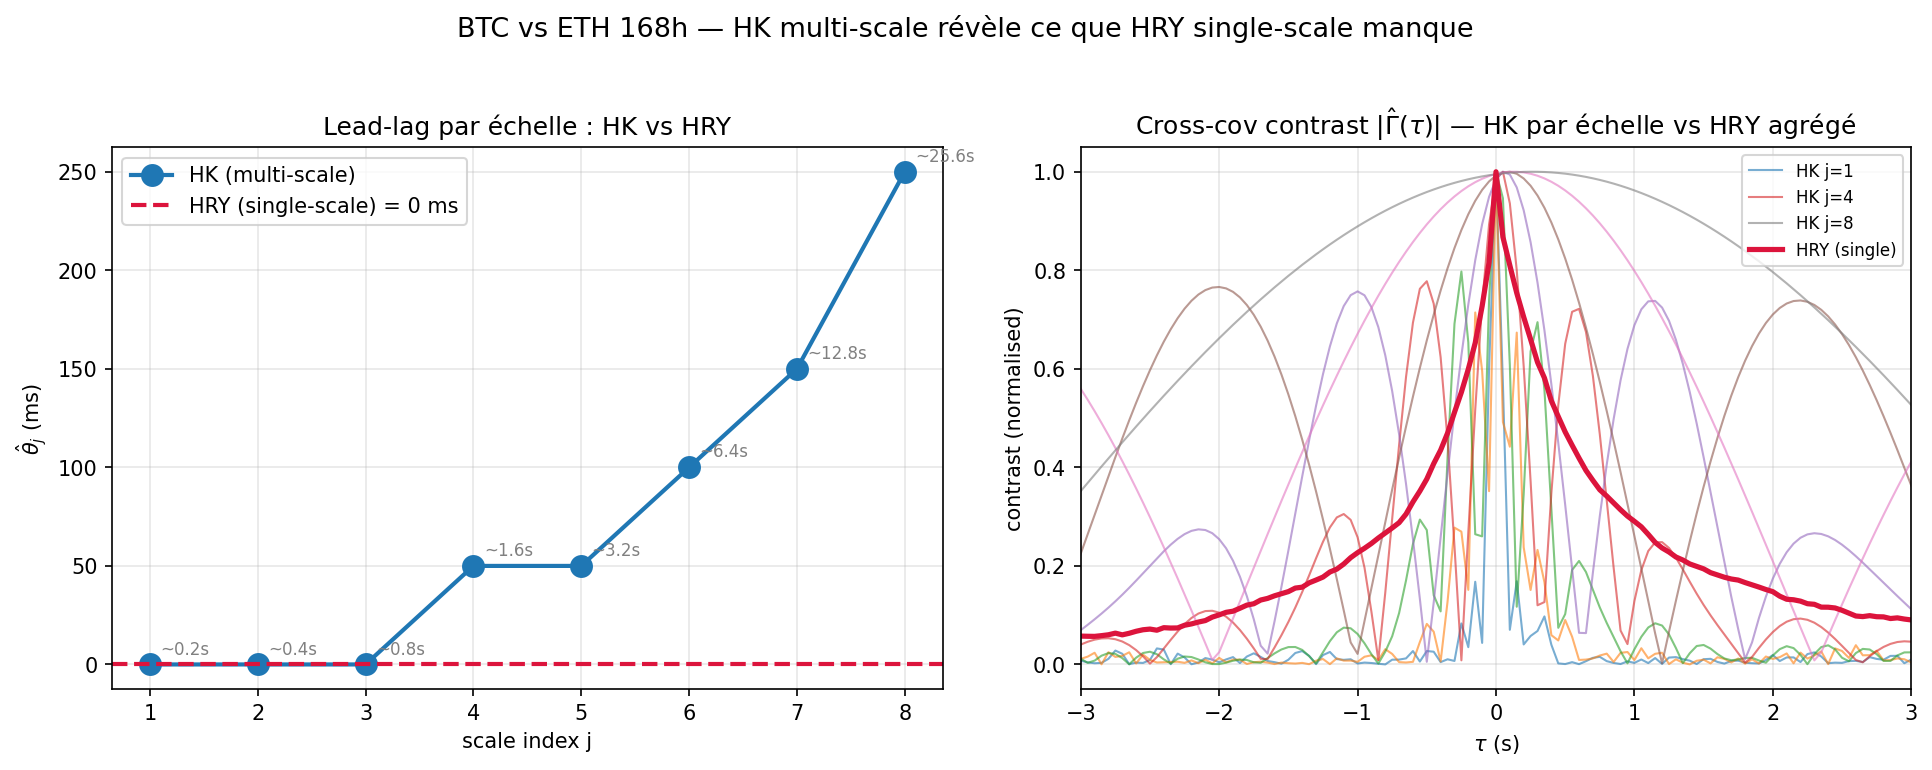
\includegraphics[width=\linewidth,height=0.68\textheight,keepaspectratio]{figures/comparison_hk_vs_hry.png}
    \end{column}
    \begin{column}{0.28\linewidth}
      \small
      \begin{block}{Exemple BTC/ETH}
        HRY renvoie un lag global proche de zéro.
      \end{block}

      \vspace{0.15cm}
      HK sépare les échelles : le profil apparaît seulement après filtrage wavelet.

      \vspace{0.15cm}
      C'est l'argument méthodologique principal du papier.
    \end{column}
  \end{columns}
\end{frame}

\begin{frame}{Extension : perpétuel vs spot}
  \begin{columns}[T]
    \begin{column}{0.49\linewidth}
      \centering
      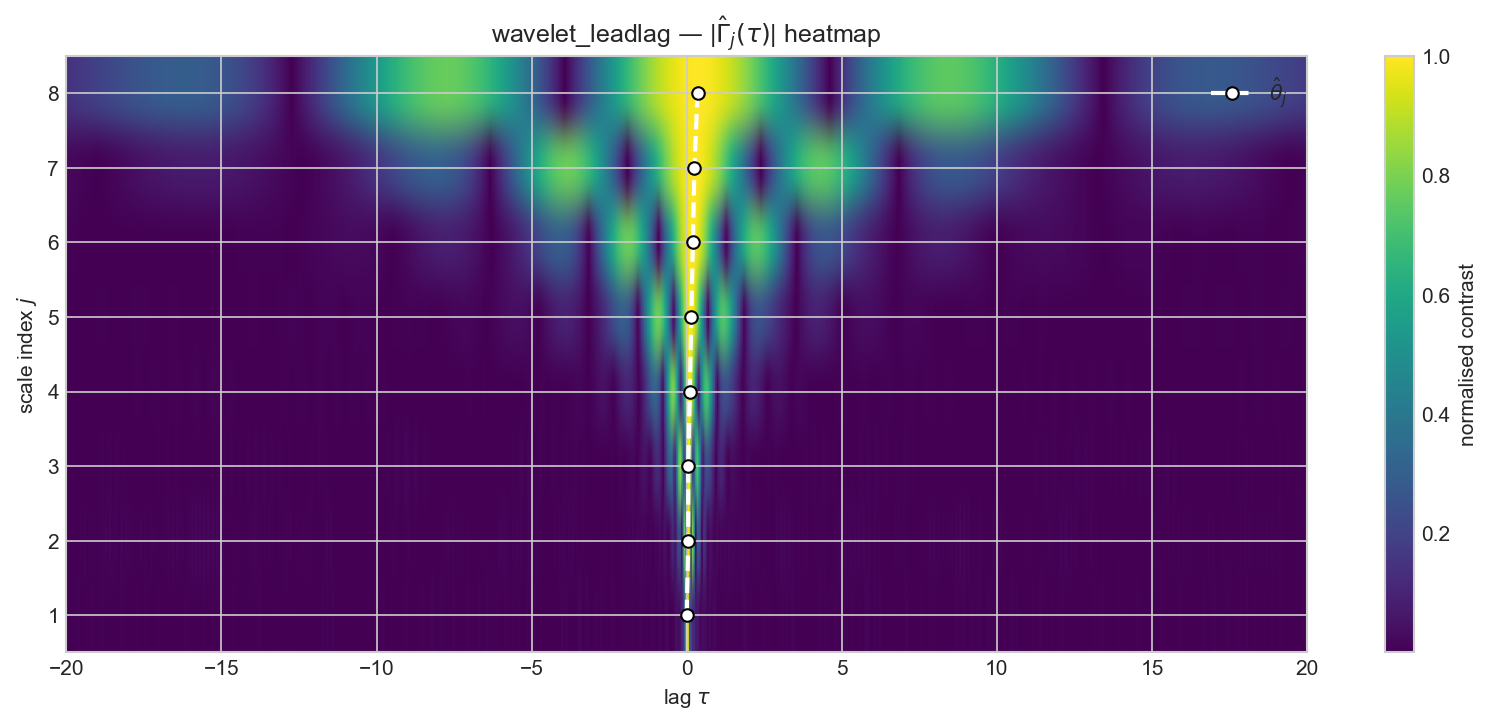
\includegraphics[width=\linewidth,height=0.56\textheight,keepaspectratio]{figures/heatmap_btc_spot_vs_perp_full_month.png}

      \small BTC : \(\hat\theta_8 = +0.35\) s
    \end{column}
    \begin{column}{0.49\linewidth}
      \centering
      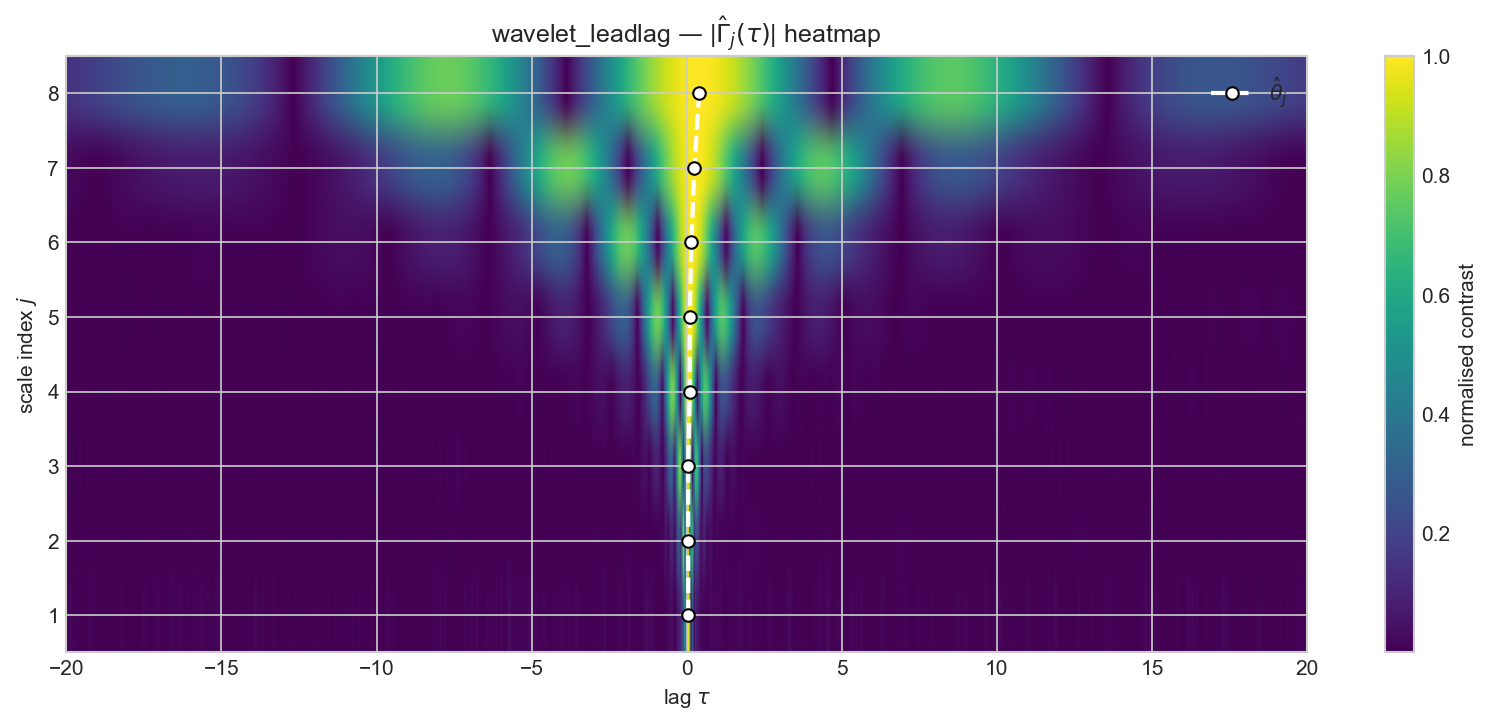
\includegraphics[width=\linewidth,height=0.56\textheight,keepaspectratio]{figures/heatmap_eth_spot_vs_perp_full_month.png}

      \small ETH : \(\hat\theta_8 = +0.40\) s
    \end{column}
  \end{columns}

  \vspace{0.2cm}
  \centering
  \textbf{Lecture :} série 1 = spot, série 2 = perpétuel ; \(\hat\theta>0\) signifie que le perpétuel mène le spot.
\end{frame}

\begin{frame}{Extension : BTC/ETH cross-asset (exploratoire)}
  \begin{columns}[T]
    \begin{column}{0.62\linewidth}
      \centering
      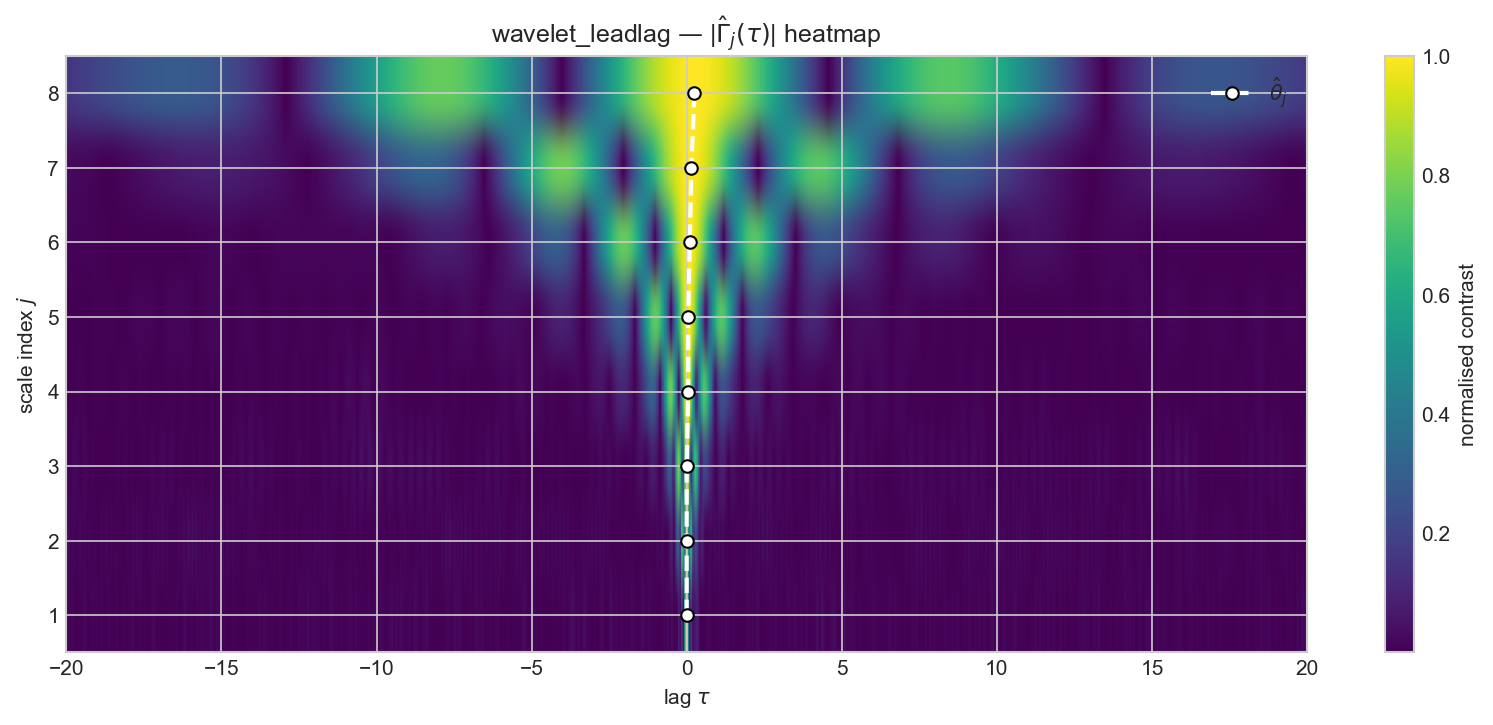
\includegraphics[width=\linewidth,height=0.66\textheight,keepaspectratio]{figures/heatmap_btc_eth_168h.png}
    \end{column}
    \begin{column}{0.34\linewidth}
      \small
      Sur aggTrades, ETH semble mener BTC aux échelles grossières : \(\hat\theta\) croît de \(+50\) à \(+250\) ms (\(j=4\) à \(8\)).
    \end{column}
  \end{columns}
\end{frame}

% ============================================================
\section{Limites et conclusion}
% ============================================================

\begin{frame}{Limites}
  \small
  \begin{tabular}{p{0.23\linewidth}p{0.68\linewidth}}
    \toprule
    \textbf{Point} & \textbf{Conséquence} \\
    \midrule
    Prix & Trades crypto au lieu des micro-prices de quotes HK. \\
    Résolution & \(\Delta_N=50\) ms : nos échelles vivent en secondes, pas en micro-latence. \\
    \bottomrule
  \end{tabular}
\end{frame}

\begin{frame}{Conclusion}
  \begin{enumerate}
    \item L'estimateur HK est réimplémenté : HY laggé, ondelette db10, argmax par échelle.
    \item Le résultat central : Binance mène Kraken sur BTC, de \(-50\) ms à \(-1.95\) s selon l'échelle.
    \item Le multi-échelle apporte quelque chose : HRY peut renvoyer zéro là où HK révèle un profil.
    \item Extesion : perpétuel vs spot solide, BTC/ETH exploratoire.
  \end{enumerate}
\end{frame}

\end{document}
